\section{项目综述}

本章节包括对云盘系统的总体介绍,包括背景介绍、功能概述、产品目标、产品结构4大部分。

\subsection{背景介绍}

现如今科学技术快速发展,大数据、深度学习、云计算等技术成为中大型企业的标配,个人用户也依赖各种云服务进行工作。然而,一切云服务都依赖于云存储技术,如果没有云存储,大量服务都将停滞无法运行。

然而,如今的云盘系统存在各种各样的问题,如不支持WebDav等文件协议、速度限制、空间有限、价格昂贵、不支持用户组之间的协作和共享等。这些问题导致目前没有一个云盘系统能够响应大部分用户的需求。

例如,个人用户期望能有一个上传、下载文件速度快,共享便利的云盘系统;企业用户期望能有一个便于团队共享、协作的云盘系统;一些特殊用户期望能有一个安全可靠、数据不外泄的云盘系统。目前云盘系统的发展仍然任重而道远。

\subsection{功能概述}

本系统将具实现如下功能:
\begin{itemize}
    \item 用户操作。注册、登录、个人信息设置、手机和电子邮箱绑定等。
    \item 文件的基本操作。文件上传、下载、移动和删除等。
    \item 好友与共享操作。添加与管理好友,文件私人共享与公共共享,共享期限和密码设置等。
    \item 文件在线操作。图片、语音、视频、文档的在线预览,图片文字识别、语音识别等。
\end{itemize}

\subsection{产品目标}

本文档致力于打造一个简单、灵活、容易扩展的云盘系统,具体来说如下:
\begin{itemize}
    \item 简单性。本系统的基本架构将只实现一些简单的操作,如上传、下载、删除、预览文件等,其余一切操作将基于可选择的插件实现。
    \item 灵活性。本系统将支持不同的主流云器务器,如NextCloud/OwnCloud/坚果云/Nginx-WebDav等,用户可自由选择。
    \item 可扩展性。本系统将支持强大的定制化服务,如功能插件、主题插件等。
\end{itemize}

\subsection{产品架构}

本系统采用微服务架构,操作对用户完全透明。其中客户端负责作为用户访问云盘服务器的接口,为用户提供可视化的交互操作;服务端负责处理业务逻辑和数据存储。

服务端内部则包括网关服务器、业务服务器、数据服务器,用户请求通过网关转发,业务服务器负责处理请求并与数据服务器交互,数据服务器负责持久化业务。数据服务器具体分为用户数据库和文件数据库,前者存储用户数据(如用户名和密码),后者用于存储文件。

\begin{figure}[H]
    \begin{center}
        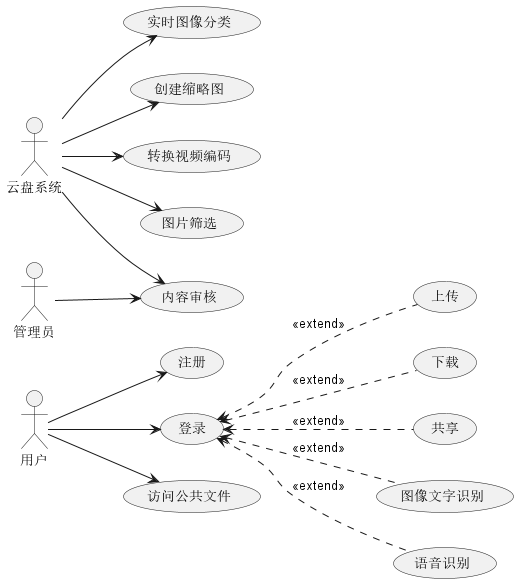
\includegraphics[scale=0.5]{examples/用例图.png}
        \caption{用例}
        \label{fig:usercase}
    \end{center}
\end{figure}

如图\ref{fig:usercase}所示,该系统中共有用户、云盘系统、管理员3个角色。其中用户可以注册、登录该系统,并在登录后进行一系列文件操作;云盘系统负责自动处理文件,如生成缩略图、智能排序、审核等操作;管理员可以对文件进行人工审核。

\begin{figure}[H]
    \begin{center}
        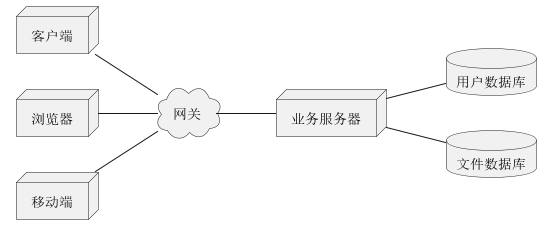
\includegraphics[scale=0.5]{examples/产品架构图.png}
        \caption{产品架构}
        \label{fig:productarch}
    \end{center}
\end{figure}

如图\ref{fig:productarch}所示,该系统由客户端、浏览器、移动端、网关、业务服务器、数据库等微服务组成。